% % Terminology collection
% irreducible - несводимый
% single entry single exit (SESE) regions of the control flow graph
% dominators
% control regions
% dominates n and b postdominates
% depth-first traversal
% we can simply visit nodes in reverse depth-first order and maintain a stack of brackets
% connecting the node to an ancestor
% lower endpoint
% brackets originating in the same subtree

% The new bracket originates from the node whose children are being merged, and extends up to the highest node whose brackets come from more than one of the branches. To add this new backedge requires keeping track (at each node in the tree) of the highest node reached by any backedge below this point. The destination of the new backedge from a node is the second"=highest of the node’s children’s highest backedges. This could be found by examination of the bracket sets, but the highest"=ending backedge is not necessarily related to the first bracket in each set (the highest"=originating), so a full search of the bracket set would be necessary.

% control dependent
% Nodes or edges
% reducible graphs
% dominance frontiers
% quick propagation graph
% use of the PST allows structure and sparsity to be exploited simultaneously
% unique entry and exit edges
% multiple edges to the entry node from outside the region, as well as out of the exit node
% bracket
% undirected graph




%% bare_conf.tex
%% V1.4b
%% 2015/08/26
%% by Michael Shell
%% See:
%% http://www.michaelshell.org/
%% for current contact information.
%%
%% This is a skeleton file demonstrating the use of IEEEtran.cls
%% (requires IEEEtran.cls version 1.8b or later) with an IEEE
%% conference paper.
%%
%% Support sites:
%% http://www.michaelshell.org/tex/ieeetran/
%% http://www.ctan.org/pkg/ieeetran
%% and
%% http://www.ieee.org/

%%*************************************************************************
%% Legal Notice:
%% This code is offered as-is without any warranty either expressed or
%% implied; without even the implied warranty of MERCHANTABILITY or
%% FITNESS FOR A PARTICULAR PURPOSE!
%% User assumes all risk.
%% In no event shall the IEEE or any contributor to this code be liable for
%% any damages or losses, including, but not limited to, incidental,
%% consequential, or any other damages, resulting from the use or misuse
%% of any information contained here.
%%
%% All comments are the opinions of their respective authors and are not
%% necessarily endorsed by the IEEE.
%%
%% This work is distributed under the LaTeX Project Public License (LPPL)
%% ( http://www.latex-project.org/ ) version 1.3, and may be freely used,
%% distributed and modified. A copy of the LPPL, version 1.3, is included
%% in the base LaTeX documentation of all distributions of LaTeX released
%% 2003/12/01 or later.
%% Retain all contribution notices and credits.
%% ** Modified files should be clearly indicated as such, including  **
%% ** renaming them and changing author support contact information. **
%%*************************************************************************


% *** Authors should verify (and, if needed, correct) their LaTeX system  ***
% *** with the testflow diagnostic prior to trusting their LaTeX platform ***
% *** with production work. The IEEE's font choices and paper sizes can   ***
% *** trigger bugs that do not appear when using other class files.       ***                          ***
% The testflow support page is at:
% http://www.michaelshell.org/tex/testflow/



\documentclass[conference]{IEEEtran}
% Some Computer Society conferences also require the compsoc mode option,
% but others use the standard conference format.
%
% If IEEEtran.cls has not been installed into the LaTeX system files,
% manually specify the path to it like:
% \documentclass[conference]{../sty/IEEEtran}

\usepackage{algorithm2e}

 % Перевод плагина
\SetKwInput{KwData}{Input parameters}
\SetKwInput{KwResult}{Result}
\SetKwInput{KwIn}{Input data}
\SetKwInput{KwOut}{Output Data}
\SetKwIF{If}{ElseIf}{Else}{if}{then}{else\ if}{else}{end\ of\ condition}
\SetKwFor{While}{while}{execute}{end\ of\ loop}
\SetKw{KwTo}{to}
\SetKw{KwRet}{return}
\SetKw{Return}{return}
\SetKwBlock{Begin}{begin\ block}{end\ block}
\SetKwSwitch{Switch}{Case}{Other}{Check\ a\ value}{and\ execute}{a\ case}{otherwise}{end\ of\ case}{end\ of\ value\ check}
\SetKwFor{For}{loop}{execute}{end\ of\ loop}
\SetKwFor{ForEach}{for\ each}{execute}{end\ of\ loop}
\SetKwRepeat{Repeat}{repeat}{while}
\SetAlgorithmName{Algorithm}{algorithm}{List of algorithms}


% Some very useful LaTeX packages include:
% (uncomment the ones you want to load)


% *** MISC UTILITY PACKAGES ***
%
%\usepackage{ifpdf}
% Heiko Oberdiek's ifpdf.sty is very useful if you need conditional
% compilation based on whether the output is pdf or dvi.
% usage:
% \ifpdf
%   % pdf code
% \else
%   % dvi code
% \fi
% The latest version of ifpdf.sty can be obtained from:
% http://www.ctan.org/pkg/ifpdf
% Also, note that IEEEtran.cls V1.7 and later provides a builtin
% \ifCLASSINFOpdf conditional that works the same way.
% When switching from latex to pdflatex and vice-versa, the compiler may
% have to be run twice to clear warning/error messages.






% *** CITATION PACKAGES ***
%
%\usepackage{cite}
% cite.sty was written by Donald Arseneau
% V1.6 and later of IEEEtran pre-defines the format of the cite.sty package
% \cite{} output to follow that of the IEEE. Loading the cite package will
% result in citation numbers being automatically sorted and properly
% "compressed/ranged". e.g., [1], [9], [2], [7], [5], [6] without using
% cite.sty will become [1], [2], [5]--[7], [9] using cite.sty. cite.sty's
% \cite will automatically add leading space, if needed. Use cite.sty's
% noadjust option (cite.sty V3.8 and later) if you want to turn this off
% such as if a citation ever needs to be enclosed in parenthesis.
% cite.sty is already installed on most LaTeX systems. Be sure and use
% version 5.0 (2009-03-20) and later if using hyperref.sty.
% The latest version can be obtained at:
% http://www.ctan.org/pkg/cite
% The documentation is contained in the cite.sty file itself.






% *** GRAPHICS RELATED PACKAGES ***
%
\ifCLASSINFOpdf
  \usepackage[pdftex]{graphicx}
  % declare the path(s) where your graphic files are
  % \graphicspath{{../pdf/}{../jpeg/}}
  % and their extensions so you won't have to specify these with
  % every instance of \includegraphics
  % \DeclareGraphicsExtensions{.pdf,.jpeg,.png}
\else
  % or other class option (dvipsone, dvipdf, if not using dvips). graphicx
  % will default to the driver specified in the system graphics.cfg if no
  % driver is specified.
  % \usepackage[dvips]{graphicx}
  % declare the path(s) where your graphic files are
  % \graphicspath{{../eps/}}
  % and their extensions so you won't have to specify these with
  % every instance of \includegraphics
  % \DeclareGraphicsExtensions{.eps}
\fi
% graphicx was written by David Carlisle and Sebastian Rahtz. It is
% required if you want graphics, photos, etc. graphicx.sty is already
% installed on most LaTeX systems. The latest version and documentation
% can be obtained at:
% http://www.ctan.org/pkg/graphicx
% Another good source of documentation is "Using Imported Graphics in
% LaTeX2e" by Keith Reckdahl which can be found at:
% http://www.ctan.org/pkg/epslatex
%
% latex, and pdflatex in dvi mode, support graphics in encapsulated
% postscript (.eps) format. pdflatex in pdf mode supports graphics
% in .pdf, .jpeg, .png and .mps (metapost) formats. Users should ensure
% that all non-photo figures use a vector format (.eps, .pdf, .mps) and
% not a bitmapped formats (.jpeg, .png). The IEEE frowns on bitmapped formats
% which can result in "jaggedy"/blurry rendering of lines and letters as
% well as large increases in file sizes.
%
% You can find documentation about the pdfTeX application at:
% http://www.tug.org/applications/pdftex





% *** MATH PACKAGES ***
%
%\usepackage{amsmath}
% A popular package from the American Mathematical Society that provides
% many useful and powerful commands for dealing with mathematics.
%
% Note that the amsmath package sets \interdisplaylinepenalty to 10000
% thus preventing page breaks from occurring within multiline equations. Use:
%\interdisplaylinepenalty=2500
% after loading amsmath to restore such page breaks as IEEEtran.cls normally
% does. amsmath.sty is already installed on most LaTeX systems. The latest
% version and documentation can be obtained at:
% http://www.ctan.org/pkg/amsmath





% *** SPECIALIZED LIST PACKAGES ***
%
%\usepackage{algorithmic}
% algorithmic.sty was written by Peter Williams and Rogerio Brito.
% This package provides an algorithmic environment fo describing algorithms.
% You can use the algorithmic environment in-text or within a figure
% environment to provide for a floating algorithm. Do NOT use the algorithm
% floating environment provided by algorithm.sty (by the same authors) or
% algorithm2e.sty (by Christophe Fiorio) as the IEEE does not use dedicated
% algorithm float types and packages that provide these will not provide
% correct IEEE style captions. The latest version and documentation of
% algorithmic.sty can be obtained at:
% http://www.ctan.org/pkg/algorithms
% Also of interest may be the (relatively newer and more customizable)
% algorithmicx.sty package by Szasz Janos:
% http://www.ctan.org/pkg/algorithmicx




% *** ALIGNMENT PACKAGES ***
%
%\usepackage{array}
% Frank Mittelbach's and David Carlisle's array.sty patches and improves
% the standard LaTeX2e array and tabular environments to provide better
% appearance and additional user controls. As the default LaTeX2e table
% generation code is lacking to the point of almost being broken with
% respect to the quality of the end results, all users are strongly
% advised to use an enhanced (at the very least that provided by array.sty)
% set of table tools. array.sty is already installed on most systems. The
% latest version and documentation can be obtained at:
% http://www.ctan.org/pkg/array


% IEEEtran contains the IEEEeqnarray family of commands that can be used to
% generate multiline equations as well as matrices, tables, etc., of high
% quality.




% *** SUBFIGURE PACKAGES ***
%\ifCLASSOPTIONcompsoc
%  \usepackage[caption=false,font=normalsize,labelfont=sf,textfont=sf]{subfig}
%\else
%  \usepackage[caption=false,font=footnotesize]{subfig}
%\fi
% subfig.sty, written by Steven Douglas Cochran, is the modern replacement
% for subfigure.sty, the latter of which is no longer maintained and is
% incompatible with some LaTeX packages including fixltx2e. However,
% subfig.sty requires and automatically loads Axel Sommerfeldt's caption.sty
% which will override IEEEtran.cls' handling of captions and this will result
% in non-IEEE style figure/table captions. To prevent this problem, be sure
% and invoke subfig.sty's "caption=false" package option (available since
% subfig.sty version 1.3, 2005/06/28) as this is will preserve IEEEtran.cls
% handling of captions.
% Note that the Computer Society format requires a larger sans serif font
% than the serif footnote size font used in traditional IEEE formatting
% and thus the need to invoke different subfig.sty package options depending
% on whether compsoc mode has been enabled.
%
% The latest version and documentation of subfig.sty can be obtained at:
% http://www.ctan.org/pkg/subfig




% *** FLOAT PACKAGES ***
%
%\usepackage{fixltx2e}
% fixltx2e, the successor to the earlier fix2col.sty, was written by
% Frank Mittelbach and David Carlisle. This package corrects a few problems
% in the LaTeX2e kernel, the most notable of which is that in current
% LaTeX2e releases, the ordering of single and double column floats is not
% guaranteed to be preserved. Thus, an unpatched LaTeX2e can allow a
% single column figure to be placed prior to an earlier double column
% figure.
% Be aware that LaTeX2e kernels dated 2015 and later have fixltx2e.sty's
% corrections already built into the system in which case a warning will
% be issued if an attempt is made to load fixltx2e.sty as it is no longer
% needed.
% The latest version and documentation can be found at:
% http://www.ctan.org/pkg/fixltx2e


%\usepackage{stfloats}
% stfloats.sty was written by Sigitas Tolusis. This package gives LaTeX2e
% the ability to do double column floats at the bottom of the page as well
% as the top. (e.g., "\begin{figure*}[!b]" is not normally possible in
% LaTeX2e). It also provides a command:
%\fnbelowfloat
% to enable the placement of footnotes below bottom floats (the standard
% LaTeX2e kernel puts them above bottom floats). This is an invasive package
% which rewrites many portions of the LaTeX2e float routines. It may not work
% with other packages that modify the LaTeX2e float routines. The latest
% version and documentation can be obtained at:
% http://www.ctan.org/pkg/stfloats
% Do not use the stfloats baselinefloat ability as the IEEE does not allow
% \baselineskip to stretch. Authors submitting work to the IEEE should note
% that the IEEE rarely uses double column equations and that authors should try
% to avoid such use. Do not be tempted to use the cuted.sty or midfloat.sty
% packages (also by Sigitas Tolusis) as the IEEE does not format its papers in
% such ways.
% Do not attempt to use stfloats with fixltx2e as they are incompatible.
% Instead, use Morten Hogholm'a dblfloatfix which combines the features
% of both fixltx2e and stfloats:
%
% \usepackage{dblfloatfix}
% The latest version can be found at:
% http://www.ctan.org/pkg/dblfloatfix




% *** PDF, URL AND HYPERLINK PACKAGES ***
%
\usepackage{url}
% url.sty was written by Donald Arseneau. It provides better support for
% handling and breaking URLs. url.sty is already installed on most LaTeX
% systems. The latest version and documentation can be obtained at:
% http://www.ctan.org/pkg/url
% Basically, \url{my_url_here}.




% *** Do not adjust lengths that control margins, column widths, etc. ***
% *** Do not use packages that alter fonts (such as pslatex).         ***
% There should be no need to do such things with IEEEtran.cls V1.6 and later.
% (Unless specifically asked to do so by the journal or conference you plan
% to submit to, of course. )


% correct bad hyphenation here
\hyphenation{op-tical net-works semi-conduc-tor}

% FIXME Remove, when got ready to publish
\usepackage[usenames,dvipsnames,svgnames,table]{xcolor}
\definecolor{rclr}{rgb}{0.5,0.1,0.1}
\definecolor{eclr}{rgb}{0,0.5,0.5}
\colorlet{acolor}{blue}
\colorlet{rcolor}{red}
\definecolor{ncolor}{rgb}{0.5,0.5,0.1}
\newcommand{\aaa}[2][acolor]{\noindent\textcolor{eclr}%
{+\ [}\textcolor{#1}{#2}\textcolor{eclr}{]}}
\newcommand{\rrr}[2][rcolor]{\noindent%
\textcolor{eclr}{-\ [}\textcolor{#1}{#2}\textcolor{eclr}{]}}
\newcommand{\nnn}[2][ncolor]{\noindent%
\textcolor{eclr}{!\ [}\textcolor{#1}{#2}\textcolor{eclr}{]}}

\begin{document}
%
% paper title
% Titles are generally capitalized except for words such as a, an, and, as,
% at, but, by, for, in, nor, of, on, or, the, to and up, which are usually
% not capitalized unless they are the first or last word of the title.
% Linebreaks \\ can be used within to get better formatting as desired.
% Do not put math or special symbols in the title.
\title{Control Flow Graph Visualization in\\ Compiled Software Engineering}


% author names and affiliations
% use a multiple column layout for up to three different
% affiliations
\author{\IEEEauthorblockN{Andrey Mikhailov${}^{*}$, Aleksey Hmelnov${}^{*}$, Evgeny Cherkashin${}^{*\;**}$ and Igor Bychkov${}^{*}$}
\IEEEauthorblockA{${}^{*}$Institute of System Dynamics and Control Theory at Siberian Branch of Russian Academy of Sciences, \\
${}^{**}$National Research Irkutsk State Technical University,\\
Irkutsk, Russian Federation\\
\texttt{\{mikhailov,alex,eugeneai,bychkov\}@icc.ru}}
}
% conference papers do not typically use \thanks and this command
% is locked out in conference mode. If really needed, such as for
% the acknowledgment of grants, issue a \IEEEoverridecommandlockouts
% after \documentclass

% for over three affiliations, or if they all won't fit within the width
% of the page, use this alternative format:
%
%\author{\IEEEauthorblockN{Michael Shell\IEEEauthorrefmark{1},
%Homer Simpson\IEEEauthorrefmark{2},
%James Kirk\IEEEauthorrefmark{3},
%Montgomery Scott\IEEEauthorrefmark{3} and
%Eldon Tyrell\IEEEauthorrefmark{4}}
%\IEEEauthorblockA{\IEEEauthorrefmark{1}School of Electrical and Computer Engineering\\
%Georgia Institute of Technology,
%Atlanta, Georgia 30332--0250\\ Email: see http://www.michaelshell.org/contact.html}
%\IEEEauthorblockA{\IEEEauthorrefmark{2}Twentieth Century Fox, Springfield, USA\\
%Email: homer@thesimpsons.com}
%\IEEEauthorblockA{\IEEEauthorrefmark{3}Starfleet Academy, San Francisco, California 96678-2391\\
%Telephone: (800) 555--1212, Fax: (888) 555--1212}
%\IEEEauthorblockA{\IEEEauthorrefmark{4}Tyrell Inc., 123 Replicant Street, Los Angeles, California 90210--4321}}




% use for special paper notices
%\IEEEspecialpapernotice{(Invited Paper)}




% make the title area
\maketitle

% As a general rule, do not put math, special symbols or citations
% in the abstract
\begin{abstract}
Engineering of the compiled software is an important task in software engineering.  One of the stages of the engineering technologies is a construction and analysis of a control flow graphs, which reflect general structures of algorithms.  The paper presents a technique for analyzing and visualizing the control flow graph of a compiled software.  The analysis is based on semantically equivalent transformations of the original graph resulting in an abstract node that contains a hierarchy of isolated regions, which then associated with predefined templates resulting a graphical representation.  The templates and additional signature data allow one to recognize the high-level programming structures and user statements to construct a flow-chart notation of the original program.

%%%% It is important stages in reverse engineering.
\end{abstract}

% no keywords

% For peer review papers, you can put extra information on the cover
% page as needed:
% \ifCLASSOPTIONpeerreview
% \begin{center} \bfseries EDICS Category: 3-BBND \end{center}
% \fi
%
% For peerreview papers, this IEEEtran command inserts a page break and
% creates the second title. It will be ignored for other modes.
\IEEEpeerreviewmaketitle

\section{Introduction}

Reverse engineering of compiled software (programs after processing its source code by a compiler) is an important task in software engineering as it allows one to solve a wide variety of software quality assessment problems, such as productivity of compiled code, quality of compiler and system libraries, peculiarities of hardware architectures the program running on.  Reverse engineering is also used for regain the access to legacy code, whose source counterpart is already lost, and for investigation of virus and malicious program behavior.  One of the helpful stages of reverse engineering techniques is a construction and analysis of so-called control flow graph that reflect a general structure of corresponding algorithms.  Artificial intelligence techniques such as pattern recognition and rewrite rule engines have extensive use in the analysis.

The control flow graph is a natural representation that can be automatically figured out from the source code or its compiled binaries.  The graph is used by compiler as an intermediate structure for optimizing transformations.  The source code text contains all the necessary information on program behavior.  Its analysis usually is a complex task even with technological support of nowadays integrated development environments, which make the analysis significantly easier.

Binary code analysis is a more complex task, and it requires a complex IT knowledge.  Special software such as disassemblers and decompilers are used to partially automatize control flow analysis and visualization.  The decompiling a binary runtime is in principle an impracticable task: the reconstructed high-level code is more difficult in understanding as compared to its assembler representation.  The visual analysis of the control flow graph is an alternate way.  There are a number of visual representation and processing software, which are relatively universal, such as uDraw (daVinci)~\cite{10}, VCG~\cite{14}, Graphlet~\cite{12}, GraVis~\cite{13}, Graph Drawing Server~\cite{9}, graphViz~\cite{11}, VisualGraph~\cite{15}.  These systems have a rich general toolkit, but visualization and analysis of control flow graph requires a special processing routines. Algorithms of graph visualization are developed since 60th~\cite{7}.  The results of P.~Eades~\cite{5}, T.~Kamada~\cite{q1}, and S.~Kawai~\cite{6} considered to be classical in this research field, they deal with universal approaches to graph visualization problems.

The control flow graph is directed and usually visualized by means of layers~\cite{4}.  The process in general consists of four stages:
\begin{itemize}
\item [] \textbf{Distribution of graph nodes between layers.} Each node is assigned a rank.  All directed edges can connect nodes from a lower rank to a higher one.  Obviously, nodes of the same rank cannot be connected with edges.  Rank distribution of the nodes is performed with various techniques, the simplest one is based on path length calculation in depth-first graph traversal procedure.
\item []\textbf{Defining order on the nodes in a layer.} The nodes of a layer are ordered according to principle of minimization of intersections of edges.  Method of median~\cite{8} is most widely used as a technique for solving the problem.
\item []\textbf{Figuring out of the node coordinates in a layer.} Each node of each layer is assigned a coordinate so as the graph will correspond to predefined aesthetic criteria.
\item []\textbf{Edge drawing.} On this stage the edges are drawn according to rules of visualization, for example, edges can be indirect lines.
\end{itemize}

The paper describes a technique and software tools for analyzing and visualizing the control flow graph of a compiled binaries.  The analysis is based on semantically equivalent transformations of the original graph resulting in a singular abstract node that contains a hierarchy of isolated regions (subgraphs).  The regions are associated with predefined templates to form resulting graphical representation.  The templates and additional signature data for library modules allow one to recognize among the regions the high-level programming language structures and statements, e.g., to construct flow-chart notation of the original program.

\section{A theoretical basis of control flow\\ graph visualization}

An directed graph $G(V,E)$ is a \emph{control flow graph} if the following restrictions hold:
\begin{enumerate}
\item graph $G$ does not contain multiple edges between the same nodes;
\item node $start\in V$ is the entrance to the graph (\emph{start node});
\item node $end \in V$ is the exit from the graph (\emph{terminal node});
\item each node $v \in V$ is accessible from $start$;
\item node $end$ is accessible from each node $v \in V$.
\end{enumerate}
If a control flow graph has more than one terminal node, the terminal nodes are connected to one new fictitious terminal node.

We will use additional notions taken from \cite{sese} and used further in the paper.  A node $x$ is a \emph{dominator} of $y$ ($x\quad dom\quad y$) in a directed graph, if any path from $start$ to $y$ includes $x$.  A node $x$ is a \emph{postdominator} of $y$ ($x\quad pdom\quad y$), if any path from $y$ to $end$ includes $x$.  By convention, a node dominates and postdominates itself.  A node $x$ is an \emph{immediate dominator} of $y$ ($x\quad idom\quad y$), if $x\quad dom\quad y$ and there are no such $p$ that $x\quad dom\quad p$ and $p\quad dom\quad y$.  A node $x$ is an \emph{immediate postdominator} of $y$ ($x\quad pidom\quad y$), if $x\quad pdom\quad y$ and there are no such $p$ that $x\quad pdom\quad p$ and $p\quad pdom\quad y$.

Let $a$ and $b$ be a pair of distinct edges in a control flow graph.  The ordered pair of $a$ and $b$ will be denoted as $\langle a,b \rangle$.  If 1) $a$ dominates $b$, 2) $b$ postdominates $a$, and c) every cycle containing $a$ also contains $b$ (and vice versa), then the pair $\langle a,b \rangle$ is referred to as a \emph{single entry single exit region} (SESE region).  In the SESE region, $a$ is the entry edge and $b$ is the exit edge.

The first condition ensures that every path from $start$ (of the whole graph) into the region passes through the entry edge $a$.  The second condition ensures that every path from inside the region to $end$ passes through the exit edge $b$.  The third condition implements two constraints: every path from inside the region to $a$ point ‘above’ $a$ passes through the exit $b$, and every path from a point ‘below’ $b$ to a point inside the region passes through the entrance $a$, i.e., these path go around the SESE region.

Two SESE regions in a control flow graph must be either folded in each other or do not overlap (contain no common nodes) \cite{sese}.  Structural analysis on the base of recognition of SESE regions commonly used for efficient construction of an intermediate image in a so called \emph{static single assignment} (SSA) form, as well as in data flow analysis.  SESE regions are also organized in \emph{program structure trees} (PST), which represent the control flow graph as hierarchy of folded regions (SESE regions and individual nodes folding tree).  Each of the PST tree nodes denote a procedure consisting of other procedures and individual operators.

A control flow graph subgraph having one entry and one exit nodes is referred to as \emph{two terminal region} (TT region).  TT regions emphasize the points of control flow convergence and the following divergence (Fig.~\ref{fig:TTRegion}).  The requirement condition of TT region recognition are weaker as compared to SESE regions, so all the SESE regions are TT regions but not vice versa.
\begin{figure}[tb]
	\centering
		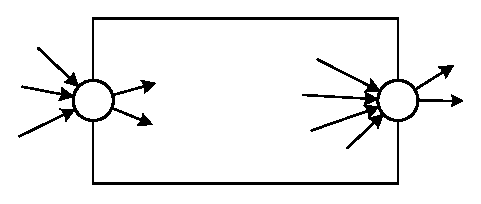
\includegraphics[width=0.4\textwidth]{Pic/TTRegion.eps}
	\caption{A two terminal region}
	\label{fig:TTRegion}
\end{figure}

For the structural programming language, TT region corresponds to a branching operator or a cycle.  Our approach to the control flow graph visualization is based on recognition of TT regions and classification them into finite set of variants concerned with various control flow operators of the original high-level programming language.  TT regions of program's graph of control flow replaced with abstract nodes (folded), giving analysis basis for visualization.

\subsection{Quality criteria of the control flow graph visualization}
\label{sec:qcrit}

A display of the nodes and the edges of a graph on a surface (or in a 3d-space) is referred to as a \emph{graph layout}.  A graph can be visualized using various layouts (Fig.~\ref{fig:VisExample}), and different layouts are defined by sets of display rules and criteria of result assessment.

\begin{figure}[b]
	\centering
		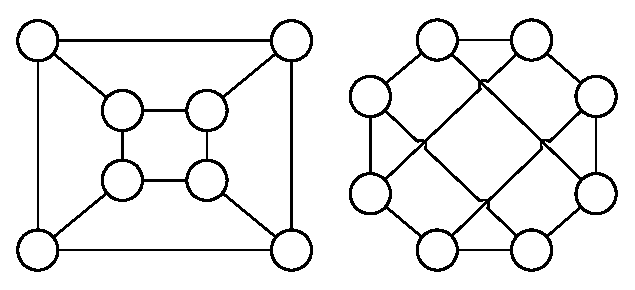
\includegraphics[width=0.4\textwidth]{Pic/Pic1.eps}
	\caption{Various layouts of the same graph}
	\label{fig:VisExample}
\end{figure}

The main quality criterion of a control graph visualization is the correspondence of the constructed image to the nature of the visualized informational object.  The quality assessment depends on various structural and semantic characteristics of the object.  Three basic feature sets are emphasized specially among the criteria: \emph{visual arrangement}, \emph{aesthetics}, \emph{restrictions}.
\begin{itemize}
\item []\textbf{Visual arrangement} is the main set of rules that a graph representation must obey to be acceptable as a desired result.  For example, to visualize programs as a flowchart, layout engine must obey agreement rules, which represent all the graph nodes as flowchart symbols and the edges as polylines consisting only with vertical and horizontal sections.  In a general case, an visual arrangement can be sufficiently complex and include a lot of details related to the target representation.
\item []\textbf{Aesthetics} is a subset of the criteria that defines attributes of the constructed image, which must be complied as much as possible to improve visibility.  A widely used aesthetic criteria are the following: minimizing a number of edge intersections, minimizing a number of foldings, minimizing the occupation area, maximizing the resolution, minimizing the total edge length, unification of edge lengths, minimizing the number of folds on an edge, foldings unification, maximizing a symmetry of graph representation, etc. % минимизация коэффициента сторон.
\item []\textbf{Restrictions} are a subset of the criteria that define layout rules for peculiar elements and subgraphs of the constructed image.  The most common used criteria are \emph{the center} that define whether the root node must be placed at the center of the image, \emph{externality} that define the necessity to place a node outside a region, \emph{cluster} defines that a number of nodes should be placed together near to each other, \emph{sequence} defines the order of nodes placement during drawing paths (left to right, top-bottom).
\end{itemize}

A control flow graph that was reconstructed from a binaries consists of operator block nodes, starting node, and an non-empty set of finish nodes, as well as edges correspond to the transfer of control.  A natural image of the control flow graph is a flowchart diagram.  For the flow charts we define the following visual arrangement for its nodes (Fig.~\ref{fig:blocks}):
\begin{itemize}
\item []\textbf{Operator shape} represents a node where the control flow passed only one direction.
\item []\textbf{Decision shape} corresponds to conditional operators in high-level programming languages; in a control flow graph it is a node, where flow control splits up.
\item []\textbf{Cycle edge shapes} denote two graph nodes, one is for beginning of the cycle and one for its end, the cycle body is located between these shapes.
\item []\textbf{Starting and terminal shapes} mark the entrance and the exit from the function or program.
\end{itemize}

\begin{figure}[b]
  \centering
  \begin{minipage}[b]{0.24\linewidth}
    \center{
\includegraphics[width=0.35\textwidth]{Pic/BlocksA.eps} \\ \footnotesize\emph{a})\\ operation}
  \end{minipage}
  \hfill
  \begin{minipage}[b]{0.24\linewidth}
    \center{
\includegraphics[width=0.35\textwidth]{Pic/BlocksB.eps} \\ \footnotesize\emph{b})\\ decision}
  \end{minipage}
  \begin{minipage}[b]{0.24\linewidth}
    \center{
\includegraphics[width=0.5\textwidth]{Pic/BlocksC.eps} \\ \footnotesize\emph{c})\\ cycle edges}
  \end{minipage}
  \begin{minipage}[b]{0.24\linewidth}
    \center{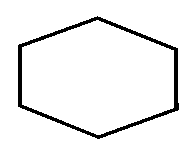
\includegraphics[width=0.35\textwidth]{Pic/BlocksD.eps} \\ \footnotesize\emph{d})\\ start/termination}
  \end{minipage}

  \caption{Types of shapes used in flow charts}
  \label{fig:blocks}
\end{figure}

In this paper, we consider a layout algorithm that visualizes control flow according to criteria defined for flowcharts.

\section{Control flow graph visualizing}
\label{sec:cfg-vis}

Nowadays programming languages in most cases contain a standard set of high-level control flow operators (\texttt{if-then}, \texttt{if-then-else}, \texttt{for}, \texttt{while}, etc.).  These operators during compilation produce their specific subgraphs.  For example, \texttt{if-then} operator produces a graph depicted in Fig.~\ref{fig:IfSt}, where \texttt{then} part could correspond to another control subgraph.
\begin{figure}[htbp]
	\centering
		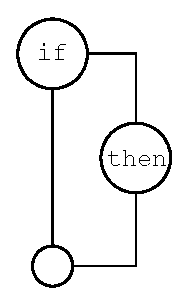
\includegraphics[width=0.11\textwidth]{Pic/Pic2.eps}
	\caption{Subgraph of \texttt{if-then} operator}
	\label{fig:IfSt}
\end{figure}

One can describe a corresponding subgraphs for all flow control operators of all standard high-level languages.  Each generated subgraph is described as a template.  The control operators are revealed and reconstructed in whole flow control graph by means of recognition of the templates in the graph and folding the recognized structure into an abstract node.  The edges terminating at and originating from the abstract node are reconnected accordingly.  The reconstruction process is repeated until either the graph folds into one abstract node, and in this case graph is referred to as \emph{reducible}, or there is a subgraph that does not correspond to any of the templates.  In the last case the graph is called \emph{inreducible}, and the subgraph that was not recognized is named \emph{undeterminate}.

Structural high-level programming language compilers produce only reducible flow control graphs.  This will hold for most of other languages as long as \texttt{goto} operator is not used explicitly or implicitly.  There are two approaches for overcoming this problem:
\begin{enumerate}
\item Perform an undeterminate subgraph riddance operation.  The essential disadvantage of the approach is the necessity of addition and deletion of nodes and edges in the graph, this is not allowed in control flow graph model visualization.
\item Recognize the undeterminate subgraph and replace it with an abstract node.
\end{enumerate}

\subsection{Algorithm of control flow graph structuring}
\label{sec:algor-contr-flow}

The developed algorithm is based on structural analysis technique proposed in~\cite{17} that suggests recognizing subgraph of a predefined form (a template) and replacing them with an abstract node, then edge endpoints reassignation is performed accordingly.  Template application is carried out according to depth-first order until the graph folds into one abstract node.  A tree of dominators is constructed.  The tree is used for edge classification and cycle recognition.  The result quality strongly depends on template application order.  The algorithm is as follows:

\begin{algorithm}[h]
\caption{Algorithm of control flow graph structuring}
\label{alg:struct}
\SetAlgoLined %% Connects logical parts with lines
\KwData{G, D, P}
\KwResult{An abstract node containing a hierarchy of folded subgraphs}
%\While{$|E| \neq 0$ и $|V| \neq 1$}{
	\ForEach{$v \in D$ in a backward breadth-first order}{
		\ForEach{$p \in Children(v)$}{
			\If{$p\quad pidom\quad v$}{
				$S \leftarrow Children(v) \setminus p $ \\
				\If{$Classify\_Region(S) \neq \textit{undeterminated}$}{
					$Apply\_Template(S)$
				}\Else{
					$Hierarchical\_Layout(S \cup p)$ \\
					$Recognize\_Undeterminanted\_Region(S)$
				}
				$Modify(G,D,P)$
			}
		}
	}
%}
\end{algorithm}

% Построим дерево доминиаторов $D$ и постдоминаторов $P$ для графа $G(E,V)$.
% In order to construct a tree of dominator $D$ and postdominator $P$.

If a program has no predefined terminating nodes, the nodes is figured out by means of the following procedure.  Firstly, the edges are categorized as \emph{forward}, \emph{backward}, and \emph{cross} directed.  Among nodes connected with forward edges, there will be at least one that has no originating edge.  If we found the only node, then the node is termination one.  Otherwise all such nodes are connected with edges to an additional fictitious termination node.  The obtained graph is correct as the termination node is accessed from any node of the graph.

Traversing of the dominator tree is done in a reverse breadth-first order, i.e. from leaves to the root, placing graph nodes in a \texttt{stack} structure.  A region having the deepest folding level (TT region) is determined on each iteration of the algorithm according to the rule $p$~$pidom$~$v$: the postdominator of node $v$ of $S$ is the terminal node, where the control flow passing $v$ converges.  This node is not added to the recognized region as it could be terminal node of other region of the graph.

%line 280 Cannot understand the essence.

As soon as a set of nodes of a TT region is recognized, the region is categorized with templates (Fig.~\ref{fig:Regions}), which are sequentially applied to it.  If the region corresponds to a template it is considered to be \emph{determined} otherwise \emph{undetermined}.

For the determined regions a new abstract node is constructed.  The node embodies its subgraphs, and bounding rectangle of the region calculated according to rules defined in the template.  The Hierarchical layout engine is applied to the undetermined regions followed by figuring out the bounding rectangle with respect to the node coordinates.  The undetermined region is replaced with new abstract node.

Finally, we obtain one abstract region, having no input and output edges.  The region will contain all the hierarchy of folded subroutines.  The bounding rectangle is figured out for the region.  All graph nodes will be located inside this rectangle.

\begin{figure}[b]
	\centering
		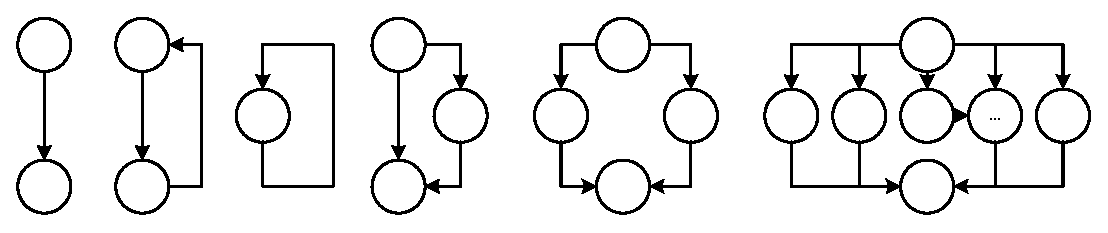
\includegraphics[width=0.49\textwidth]{Pic/Reg.eps}
	\caption{Applicable templates}
	\label{fig:Regions}
\end{figure}

\subsection{Layout engine}
\label{sec:raskladka-process}

The layout process is carried out recursively from top region down to lower regions.  For the top region initial coordinates is predefined.  If a region has a template with visualization rules, the rules are applied.  The layout example if \texttt{if-then-else} operator is given in Fig.~\ref{fig:IfThenElse}.

\begin{figure}[b]
	\centering
		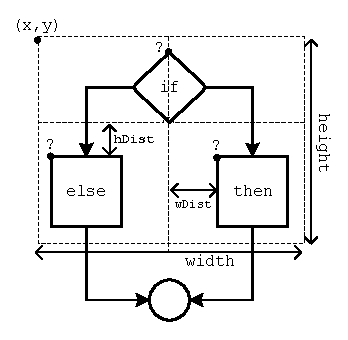
\includegraphics[width=0.3\textwidth]{Pic/IfThenElse.eps}
	\caption{Visualizing template of \texttt{if-then-else} operator}
	\label{fig:IfThenElse}
\end{figure}

The coordinate computation rules for \texttt{if-then-else} operator is as follows:
\begin{itemize}
\item [] \texttt{if.x = x + abs(width - if.width) / 2};
\item [] \texttt{then.x = x  + wDist / 2, then.y = y + if.height + hDist};
\item [] \texttt{else.x = x - else.width - wDist / 2, else.y = y + if.height + hDist};
\end{itemize}
where \texttt{wDist} is a vertical distance between nodes, \texttt{hDist} is a horizontal distance.  These parameters is defined manually and reflect aesthetic criteria.  The visualizing rules are defined analogously for each template.  Thus, the layout engine consists of sequential applications of the visualizing rules to the folded regions.

\section{Implementation}
\label{sec:implementation}

The algorithm is implemented in the Java programming language.  The main application is named ``VisualGraph'' and implemented using authors' library ``JGraphX'' containing the subroutines of the algorithm.  The application uses hierarchical graph models for the control flow visualization using authors' and other known popular visualization algorithms.  The ``JGraphX'' library allows one to make images of control flow graphs, defining shapes and colors for nodes, draw edges between nodes and corner points automatically and manually.

At present the library and application support some visual arrangement criteria from section \ref{sec:qcrit}.  Categorization of nodes in branching regions of the control flow graph requires that the graph will be attributive and contain assembler code of the main program blocks (lineal parts of code).  The control flow graph itself is obtained from assembler program semantics analysis by means of authors FlexT based utilities \cite{flext}.

% An example of a floating figure using the graphicx package.
% Note that \label must occur AFTER (or within) \caption.
% For figures, \caption should occur after the \includegraphics.
% Note that IEEEtran v1.7 and later has special internal code that
% is designed to preserve the operation of \label within \caption
% even when the captionsoff option is in effect. However, because
% of issues like this, it may be the safest practice to put all your
% \label just after \caption rather than within \caption{}.
%
% Reminder: the "draftcls" or "draftclsnofoot", not "draft", class
% option should be used if it is desired that the figures are to be
% displayed while in draft mode.
%
%\begin{figure}[!t]
%\centering
%\includegraphics[width=2.5in]{myfigure}
% where an .eps filename suffix will be assumed under latex,
% and a .pdf suffix will be assumed for pdflatex; or what has been declared
% via \DeclareGraphicsExtensions.
%\caption{Simulation results for the network.}
%\label{fig_sim}
%\end{figure}

% Note that the IEEE typically puts floats only at the top, even when this
% results in a large percentage of a column being occupied by floats.


% An example of a double column floating figure using two subfigures.
% (The subfig.sty package must be loaded for this to work.)
% The subfigure \label commands are set within each subfloat command,
% and the \label for the overall figure must come after \caption.
% \hfil is used as a separator to get equal spacing.
% Watch out that the combined width of all the subfigures on a
% line do not exceed the text width or a line break will occur.
%
%\begin{figure*}[!t]
%\centering
%\subfloat[Case I]{\includegraphics[width=2.5in]{box}%
%\label{fig_first_case}}
%\hfil
%\subfloat[Case II]{\includegraphics[width=2.5in]{box}%
%\label{fig_second_case}}
%\caption{Simulation results for the network.}
%\label{fig_sim}
%\end{figure*}
%
% Note that often IEEE papers with subfigures do not employ subfigure
% captions (using the optional argument to \subfloat[]), but instead will
% reference/describe all of them (a), (b), etc., within the main caption.
% Be aware that for subfig.sty to generate the (a), (b), etc., subfigure
% labels, the optional argument to \subfloat must be present. If a
% subcaption is not desired, just leave its contents blank,
% e.g., \subfloat[].


% An example of a floating table. Note that, for IEEE style tables, the
% \caption command should come BEFORE the table and, given that table
% captions serve much like titles, are usually capitalized except for words
% such as a, an, and, as, at, but, by, for, in, nor, of, on, or, the, to
% and up, which are usually not capitalized unless they are the first or
% last word of the caption. Table text will default to \footnotesize as
% the IEEE normally uses this smaller font for tables.
% The \label must come after \caption as always.
%
%\begin{table}[!t]
%% increase table row spacing, adjust to taste
%\renewcommand{\arraystretch}{1.3}
% if using array.sty, it might be a good idea to tweak the value of
% \extrarowheight as needed to properly center the text within the cells
%\caption{An Example of a Table}
%\label{table_example}
%\centering
%% Some packages, such as MDW tools, offer better commands for making tables
%% than the plain LaTeX2e tabular which is used here.
%\begin{tabular}{|c||c|}
%\hline
%One & Two\\
%\hline
%Three & Four\\
%\hline
%\end{tabular}
%\end{table}


% Note that the IEEE does not put floats in the very first column
% - or typically anywhere on the first page for that matter. Also,
% in-text middle ("here") positioning is typically not used, but it
% is allowed and encouraged for Computer Society conferences (but
% not Computer Society journals). Most IEEE journals/conferences use
% top floats exclusively.
% Note that, LaTeX2e, unlike IEEE journals/conferences, places
% footnotes above bottom floats. This can be corrected via the
% \fnbelowfloat command of the stfloats package.


\section{A layout example}

Let's consider a result of our algorithm in comparison to one of hierarchic layout engines (Fig.~\ref{fig:image1}).  In the figure, our algorithm (\emph{a}) specially emphasizes the backward edge that corresponds to a loop.  The edge style is visually distinguishable from other edges.  The algorithm also marks the terminal nodes.  Such visualization features allow to recognize visually the regions of interest and other kinds of analysis.  In Fig.~\ref{fig:image1}\emph{а}, the edges are represented with straight plain lines (except edge connecting \texttt{v9} and \texttt{v5}).  This will ease of control transferring analysis as compared to the form in Fig.~\ref{fig:image1}\emph{б}. Note, that the proposed algorithm accounts not all the variants of control flow patterns and can be improved for example to support undetermined edges removal in a region.

%  а) иерархический, б) структурный
% fig
\begin{figure}[b]
	\begin{minipage}[b]{0.49\linewidth}
	\center{\includegraphics[width=0.75\textwidth]{Pic/Hgraph.pdf} \\\footnotesize \emph{a}) hierarchical}
	\end{minipage}
\hfill
\begin{minipage}[b]{0.49\linewidth}
	\center{\includegraphics[width=0.94\textwidth]{Pic/Sgraph.pdf} \\\footnotesize \emph{b}) structural}
	\end{minipage}
	\caption{Layouts of a control flow graph}
	\label{fig:image1}
\end{figure}


\section{Conclusion}
We have proposed and implemented a software tools realizing an approach to surface graph layout on the base of techniques of structural analysis.  The main difference of our approach as compared to the mentioned (in the paper) techniques is the usage of a set of matching rules, which are applied to two two terminal nodes (a special subgraph) to recognize original control flow structures of high-level programming language.

A probation of the developed algorithms was performed on CPU2000 test set\footnote{https://www.spec.org/cpu2000/ --- Standard Performance Evaluation Corporation.  SPEC CPU2000 is a test set for assessment of the performance of a central processing unit. The test are used for compiler quality evaluation.}.  The following results are obtained:
\begin{itemize}
\item 197.parser (Syntactic parser of a natural language);
\item 252.eon (Ray tracing).
\end{itemize}

The automation of the flow control analysis allows an engineer to devote more efforts for description of the templates increasing both the personal productivity and detail level of the software description.

The results of the control flow graph analysis could be used in construction of Model driven engineering (MDE)~\cite{mda} software development tools.  The nowadays approaches to MDE is based on change propagation between various models of the software, e.g., source code generation from UML and BPMN2.0, and (in backward direction) refactoring the high-level models according to local source code modification.  Comparing results of control flow graph analysis could determine initial change of the structure of the source code, then the change is propagated to the higher-level models.  This is however a very complex fundamental problem containing both deduction and induction logical inferences.

% conference papers do not normally have an appendix

% use section* for acknowledgment
\section*{Acknowledgment}

\aaa{The results presented in the paper are obtained with partial support of...
The authors would like to thank...}








% trigger a \newpage just before the given reference
% number - used to balance the columns on the last page
% adjust value as needed - may need to be readjusted if
% the document is modified later
%\IEEEtriggeratref{8}
% The "triggered" command can be changed if desired:
%\IEEEtriggercmd{\enlargethispage{-5in}}

% references section

% can use a bibliography generated by BibTeX as a .bbl file
% BibTeX documentation can be easily obtained at:
% http://mirror.ctan.org/biblio/bibtex/contrib/doc/
% The IEEEtran BibTeX style support page is at:
% http://www.michaelshell.org/tex/ieeetran/bibtex/
%\bibliographystyle{IEEEtran}
% argument is your BibTeX string definitions and bibliography database(s)
%\bibliography{IEEEabrv,../bib/paper}
%
% <OR> manually copy in the resultant .bbl file
% set second argument of \begin to the number of references
% (used to reserve space for the reference number labels box)
\begin{thebibliography}{9}

\bibitem{10} M.~Frohlich, M.~Werner, \emph{Demonstration of the Interactive Graph Visualization System daVinci}, LNCS~894, 1995,~P.~266--269.

\bibitem{14} G.~Sander, \emph{Graph loyout through the VCG tool}, LNCS~894, 1995, P.~194--205.

\bibitem{12} M.~Himsolt, \emph{Graphlet System (System Demonstration)}, LNCS~1990, 1996. P.~233--240.

\bibitem{13} H.~Lauer, M.~Ettrich, K.~Soukup, \emph{GraVis System Demonstration}, LNCS~1353, 1997, P.~344--349.

\bibitem{9} S.~Bridgeman, A.~Garg, R.~Tamassia, \emph{A Graph Drawing and Translation Service on the WWW}, LNCS~1190, 1996, P.~45--52.

\bibitem{11} E.~R.~Gasner, S.~C.~North, \emph{An Open Graph Visualization System and its Applications to Software Engineering}, \url{http://www.graphviz.org/Documentation/GN99.pdf}

\bibitem{15} T.~A.~Zolotukhin, \emph{Graph Visualization with Programming System ``Visual Graph''}, Computer Science in Science and Education, 2012, P.~135--148. (in~Russian)

\bibitem{18} A.~A.~Mikhailov, \emph{Control Flow Graph Analysis in Decompilation of Object Files dcuil}, Vestnik of Novosibirsk State University, Computer Science Technologies Series, 2014, Vol.~12, Issue~2, P.~74--79. (in~Russian)

\bibitem{1} V.~N.~Kasyanov, \emph{Visualizing Information on the Base of Graph Models}, Computational Technologies, 1999. Vol.~11, No.~11, P.~1123--1135. (in~Russian)

\bibitem{7} W.~T.~Tutte, \emph{How to Draw a Graph}, Proc. of London Math. Society. 1963. 13(52),  P.~743--768.

\bibitem{5} P.~A.~Eades, \emph{A Heuristic for Graph Drawing}, Congressus Numerantium, 1984, 42,  P.~149--160.

\bibitem{6} T.~Kamada, S.~Kawai, \emph{An Algorithm for Drawing General Undirected Graphs}, Inform. Process. Lett, 1989, 31, P.~7--15.

\bibitem{4} P.~Eades, L.~Xuemin, \emph{How to Draw a Directed Graph}, Visual Languages, 1989, IEEE Workshop on, IEEE, 1989, P.~13--17.

\bibitem{8} P.~Eades, N.~C.~Wormald, \emph{The Median Heuristic for Drawing 2--Layered Networks}, Technical Report 69, Dept. of Computer Science, University of Queensland, 1986.

\bibitem{16} A.~V.~Aho, R.~Sethi, J.~D.~Ullman, \emph{Compilers: Principles, Techniques, And Tools}, Addison Wesley, 1986.  MLA

\bibitem{17} C.~Cifuentes, \emph{Structuring Decompiled Graphs. Compiler Construction}, Springer Berlin Heidelberg, 1996, P.~91--105.

\bibitem{3} R.~Johnson,D.~Pearson, and K.~Pingali, \emph{Finding regions fast: Single entry single exit and control regions in linear time}. Tech. rep., Cornell University, Ithaca, NY, 1993

\bibitem{sese} R.~Johnson, D.~Pearson, K.~Pingali, \emph{The Program Structure Tree: Computing Control Regions in Linear Time}, In PLDI '94: Proceedings of the ACM SIGPLAN 1994 conference on Programming language design and implementation, New York, NY, USA, 1994. ACM. p.~171--185. \url{http://iss.ices.utexas.edu/Publications/Papers/PLDI1994.pdf} (access data: 12.02.2016)

\bibitem{flext} A.~Hmelnov, S.~Vassilyev, \emph{Data description language FlexT: flexible types for description of static data}, Proceedings of CSCC'99 Multiconference. P.~1371-1376 URL:\url{http://www.wseas.us/e-library/conferences/athens1999/Papers/137.pdf} (access date: 12.01.2016)
\bibitem{mda} E.~A.~Cherkashin, V.~V.~Paramonov, et al, \emph{Model Driven Architecture is a Complex System}. E-Society Journal Research and Applications 2 (2), 15--23.


%\bibitem{IEEEhowto:kopka}
%H.~Kopka and P.~W. Daly, \emph{A Guide to \LaTeX}, 3rd~ed.\hskip 1em plus
%  0.5em minus 0.4em\relax Harlow, England: Addison-Wesley, 1999.

\end{thebibliography}




% that's all folks
\end{document}

%%% Local Variables:
%%% mode: latex
%%% TeX-master: t
%%% End:
